\documentclass{beamer}
\usepackage[utf8]{inputenc}

\usetheme{Madrid}
\usecolortheme{default}
\usepackage{amsmath,amssymb,amsfonts,amsthm}
\usepackage{txfonts}
\usepackage{tkz-euclide}
\usepackage{listings}
\usepackage{adjustbox}
\usepackage{array}
\usepackage{tabularx}
\usepackage{gvv}
\usepackage{lmodern}
\usepackage{circuitikz}
\usepackage{tikz}
\usepackage{graphicx}

\setbeamertemplate{page number in head/foot}[totalframenumber]

\usepackage{tcolorbox}
\tcbuselibrary{minted,breakable,xparse,skins}



\definecolor{bg}{gray}{0.95}
\DeclareTCBListing{mintedbox}{O{}m!O{}}{%
  breakable=true,
  listing engine=minted,
  listing only,
  minted language=#2,
  minted style=default,
  minted options={%
    linenos,
    gobble=0,
    breaklines=true,
    breakafter=,,
    fontsize=\small,
    numbersep=8pt,
    #1},
  boxsep=0pt,
  left skip=0pt,
  right skip=0pt,
  left=25pt,
  right=0pt,
  top=3pt,
  bottom=3pt,
  arc=5pt,
  leftrule=0pt,
  rightrule=0pt,
  bottomrule=2pt,
  toprule=2pt,
  colback=bg,
  colframe=orange!70,
  enhanced,
  overlay={%
    \begin{tcbclipinterior}
    \fill[orange!20!white] (frame.south west) rectangle ([xshift=20pt]frame.north west);
    \end{tcbclipinterior}},
  #3,
}
\lstset{
    language=C,
    basicstyle=\ttfamily\small,
    keywordstyle=\color{blue},
    stringstyle=\color{orange},
    commentstyle=\color{green!60!black},
    numbers=left,
    numberstyle=\tiny\color{gray},
    breaklines=true,
    showstringspaces=false,
}
%------------------------------------------------------------

\title
{2.2.16}
\author 
{AI25BTECH11023 - Pratik R}



\begin{document}

\frame{\titlepage}
\begin{frame}{Question}

 The angle between the planes
$$
\vec r \cdot (2\hat{i}-3\hat{j}+\hat{k})=1 \text{ and } 
$$
$$
\vec r \cdot(\hat{i}-\hat{j})=4
$$   

\end{frame}

    

\section{Solution}
\begin{frame}{Solution}
\textbf{Solution:} 
\\
Let $P_1$ and $P_2$ are the planes given respectively. \\
The normal vector of the planes, say $n_1$ and $n_2$ are:
\begin{align}
    \vec {n_1}= \myvec{2 \\ -3 \\ 1} \\
    \vec {n_1}= \myvec{1 \\ -1 \\ 0}
\end{align}

Thus, the cosine of the angle between the two is


\begin{align}
   \cos \theta = \frac{\vec {n_1} \cdot \vec {n_1}}{|n_1||n_2|}  
\end{align}
\begin{align}
    = \frac{5}{\sqrt{14}\times\sqrt{2}} = \frac{5}{\sqrt{28}}
\end{align}
\begin{align}
    \implies \theta = \cos ^{-1}\frac{5}{\sqrt{28}}
\end{align}
where $\theta$ is the acute angle between the planes.

    \end{frame}
    \subsection{plot}
       \begin{frame}[fragile]
    \begin{figure}[H]
    \centering
    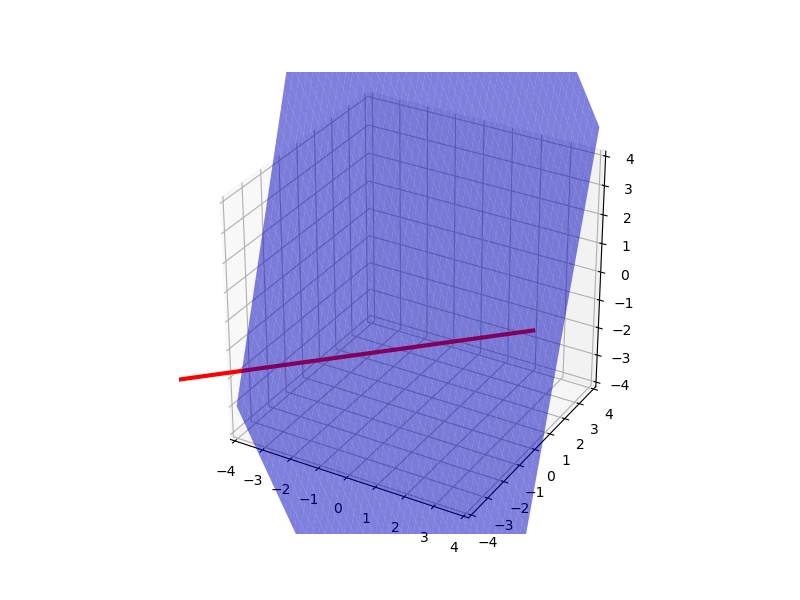
\includegraphics[width = 0.6\columnwidth]{../figs/fig.png}
    \caption*{}
    \label{figs}
\end{figure}
\end{frame}

\end{document}
